\section{Getting Quantitative: New Thermal Properties}
\label{act1.2.1}

\begin{overview}

\noindent
{\bfseries Overview:} So far, we've used qualitative descriptions and we've estimated numbers to describe the thermal phenomena occurring in the heat pack. However, we often need to be able to accurately quantify our observations and come up with mathematical models that can hopefully give us precise predictions for measurements. In this section, we'll familiarize ourselves with some mathematical models for thermal properties. In particular, we'll talk about \emph{Heat Capacity and Specific Heat,} as well as \emph{Heat of Vaporization} and \emph{Heat of Melting}.

\end{overview}

\note{Timing: \unit[$\sim$30]{min}}{

	\subsubsection*{Purpose}
		\begin{itemize}
			\item To provide an opportunity to become familiar and comfortable using the constructs heat capacity, molar heat capacity, specific heat, and heats of vaporization and melting and how these constructs relate to the previously used constructs in the \ThreePhaseModel{} and \EnergyInteractionModel{}
		\end{itemize}
		
		This activity takes the qualitative analysis the students know how to do and makes it quantitative by incorporating the actual specific heats and heats of melting, etc.\ for specific substances. It also clarifies the difference between the intensive quantities of specific heats and the extensive quantity heat capacity. Similarly for $\Delta H$. The units used with $\Delta H$ (intensive quantity) or with lower case c (specific heat), clarify how to convert the intensive quantity to the extensive quantity that is usually of interest. Note: We consciously use notation that these particular students are most likely to come across in their chemistry and biology texts.
	
	\subsubsection*{Learning Outcomes}
		\begin{itemize}
			\item Understand and be able to describe/explain the constructs of heat capacity, heat, and a change in temperature.
			\item Understand and be able to describe/explain the connection between heat capacity and thermal energy.
			\item Understand and be able to describe/explain the difference between heat capacity, molar heat capacity, and specific heat and know how to decide when to use which one.
			\item Understand and be able to describe/explain how $\left|\Delta H_\text{VAP}\right|$ and $\left|\Delta H_\text{MELT}\right|$ connect to $\Delta E_\text{BOND}$.
		\end{itemize}
}


\noindent Your instructor will give you one or two minutes to discuss each of the following in the following parts~\hyperref[1.2.1A]{\ref*{1.2.1A}} and \ref{1.2.1B} in your Small Groups. Quickly come to a consensus and put your response on the board. Each question will be followed by a brief \framebox[1.1\width][c]{\textbf{Whole Class Discussion}}.

\subsection{Heat Capacity}
\label{1.2.1A}

\begin{enumerate}
	\item You may have used the relationship \framebox{$Q = C\Delta T$} in chemistry and physical science classes. \textbf{What does ``heat capacity'' mean \emph{in your own words?}} You don't have to put this on the board, but make sure everyone in your group is ready to explain.
		
	\note{}{
		Try to get answers that are not simply a restatement of an equation. ``Heat capacity,'' as all concepts, has a deeper meaning than an expression in a certain set of units. For example, an appropriate answer here might be: ``Heat capacity is a measure of the amount of heat that must be added to an object to raise its temperature; the greater the heat capacity, the more heat that must be added to raise an object's temperature a certain amount.''  
	}
		
	\item Imagine you have a big bucket of water and a small (like, European-sized) teacup of water, which would have the greater heat capacity -- the water in the bucket or in the teacup? Which would have the greater specific heat?
		
	\note{}{
		Bucket has much larger heat capacity, due to much larger quantity of water. Since both substances are the same, they have the same specific heat. This is an example of the difference between extensive and intensive quantities.
	}
		
	\item Create an \emph{open-system \EnergyDiagram{}} that illustrates the process of making a heat capacity measurement for the big bucket of water (adding heat to this water).\\
	\textbf{Note:} We are assuming that this measurement takes place at a \emph{constant volume} (no water is lost during the measurement). The significance of this will make more sense later in the course.
	\label{1.2.1A3}
		
	\note{}{
		\noindent
		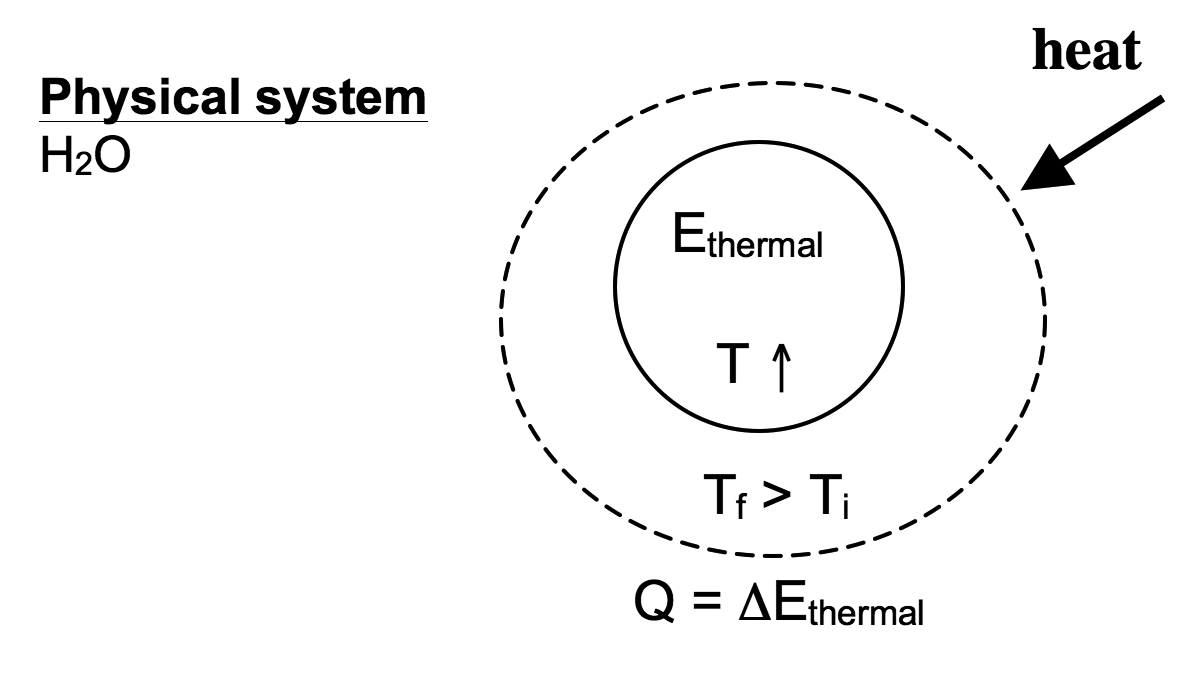
\includegraphics[width=\linewidth]{act121-3}
	}
		
	\item Use your diagram from (3) and the definition of heat capacity to develop an algebraic relationship that relates change in thermal energy to temperature change and heat capacity.
		
	\note{}{
		$\Delta E_\text{thermal} = C \Delta T$
		
		[$C$ units are \unitfrac[]{J}{K}    units for $\Delta T$ can be in either Celsius orr $KE$lvin, since the size of the degree is the same]
	}
		
	\item Use the following definitions to determine simple algebraic relationships between the heat capacity and each of two specific heats (mass \& molar): 
	
	\begin{itemize}
		\item Mass specific heat is the heat capacity per kilogram,
		
		\textbf{and}
		
		\item Molar specific heat is the heat capacity per mole.
	\end{itemize}	

	In what situations would one or the other be more useful or convenient to use?
		
	\note{}{
		Mass specific heat, $c_m = \nicefrac{C}{m}$; $m$ is mass.
		
		Molar specific heat, $c_n = \nicefrac{C}{n}$; $n$ is \# of moles.
	}
\end{enumerate}

\subsection{Heat of Vaporization and Heat of Melting}
\label{1.2.1B}

\begin{enumerate}
	\item You may have used the relationship \framebox{$Q = \Delta H$} in chemistry and physical science classes. \textbf{What does ``heat of melting'' -- or ``heat of vaporization'' -- mean \emph{in your own words?}} As above, you don't have to put this on the board, but you should make sure everyone in your group is ready to explain.
	\label{1.2.1B1}
	
	\note{}{
		They should say something like, ``Heat of vaporization'' is a measure of the amount of heat that must be added to a substance to totally vaporize it.
	}
	
	\item Use the \EnergyInteractionModel{} to illustrate a process in which $Q = \Delta E_\text{BOND}$.
	
	\note{}{Same as \hyperref[1.2.1A3]{\S\ref*{1.2.1A}\#3}, with bond energy instead of thermal energy.}
	
	\item If $\left|\Delta H\right|$ were given in units of joules per kilogram (\unitfrac[]{J}{kg}) or units of joules per mole (\unitfrac[]{J}{mol}), instead of units of joules, how would the equation, $Q = \Delta H$, change?
	\label{1.2.1B3}
	
	\note{}{
		$Q = \pm \left|\Delta H\Delta m\right|$, where $\Delta m$ means the amount of mass that changed phase; similarly for units of joules/mole, with $\Delta n$ instead of $\Delta m$. 
		
		This gets at the distinction between intensive and extensive quantities. To change an intensive quantity to an extensive quantity, such as $\Delta H$ as it is used in \hyperref[1.2.1B1]{\S\ref*{1.2.1B}\#1} (where it has units of joules), you have to multiply by the amount of the substance in the units the intensive quantity is expressed in. The two expressions in \hyperref[1.2.1B3]{\S\ref*{1.2.1B}\#3} are the most common intensive expressions for $\Delta H$. When $\Delta H$ is used as an intensive quantity, it would typically have a subscript, such as $\Delta H_\text{vap}$, but this is not a hard and fast rule and $\Delta H$ as an extensive quantity could also be subscripted. You and your students need to always be aware of the specific context.
	}
	
	\item Use questions 1 through 3 above to describe a specific relationship between the change in bond energy in our \EnergyInteractionModel{}, and the indicator of the bond energy system (i.e., the portion of mass of a substance that changed phase).
	
	\note{}{$\Delta E_\text{bond} = \pm\left|\Delta m \Delta H \right|$}
	
	\item Rewrite the equation expressing energy conservation for process (b) in \ref{fnt1.1.3-2}, using the expressions for $\Delta E_\text{th}$ and $\Delta E_\text{BOND}$ that were introduced in this activity in terms of C and H. Then substitute all known values for each variable in your expression.

\end{enumerate}

	\noindent\textbf{Let's think about our heat pack again:} What information do you need to determine how much mass will change phase when the button is clicked, assuming the heat pack is completely thermally insulated?

\WCD

	\note{Purpose}{
		To connect these new, quantitative expressions to the diagrams they have just learned to make
		\begin{align*}
			\Delta E_\text{th} + \Delta E_\text{bond} \&= 0\\
			C\Delta T - \left| \Delta m \Delta H \right| \&= 0\\
			C(54^\circ C - 23^\circ C) - \left| \Delta m \Delta H \right| \&= 0.
		\end{align*}
		They only need values for $C$ and $\Delta H$. Make sure students check that the signs of the terms make sense. 
		}